\documentclass[14pt]{extreport}
\usepackage{gost}

\usepackage{mathtools}
\usepackage{minted}
\usepackage{booktabs}
\usepackage{xcolor}

\begin{document}
	
	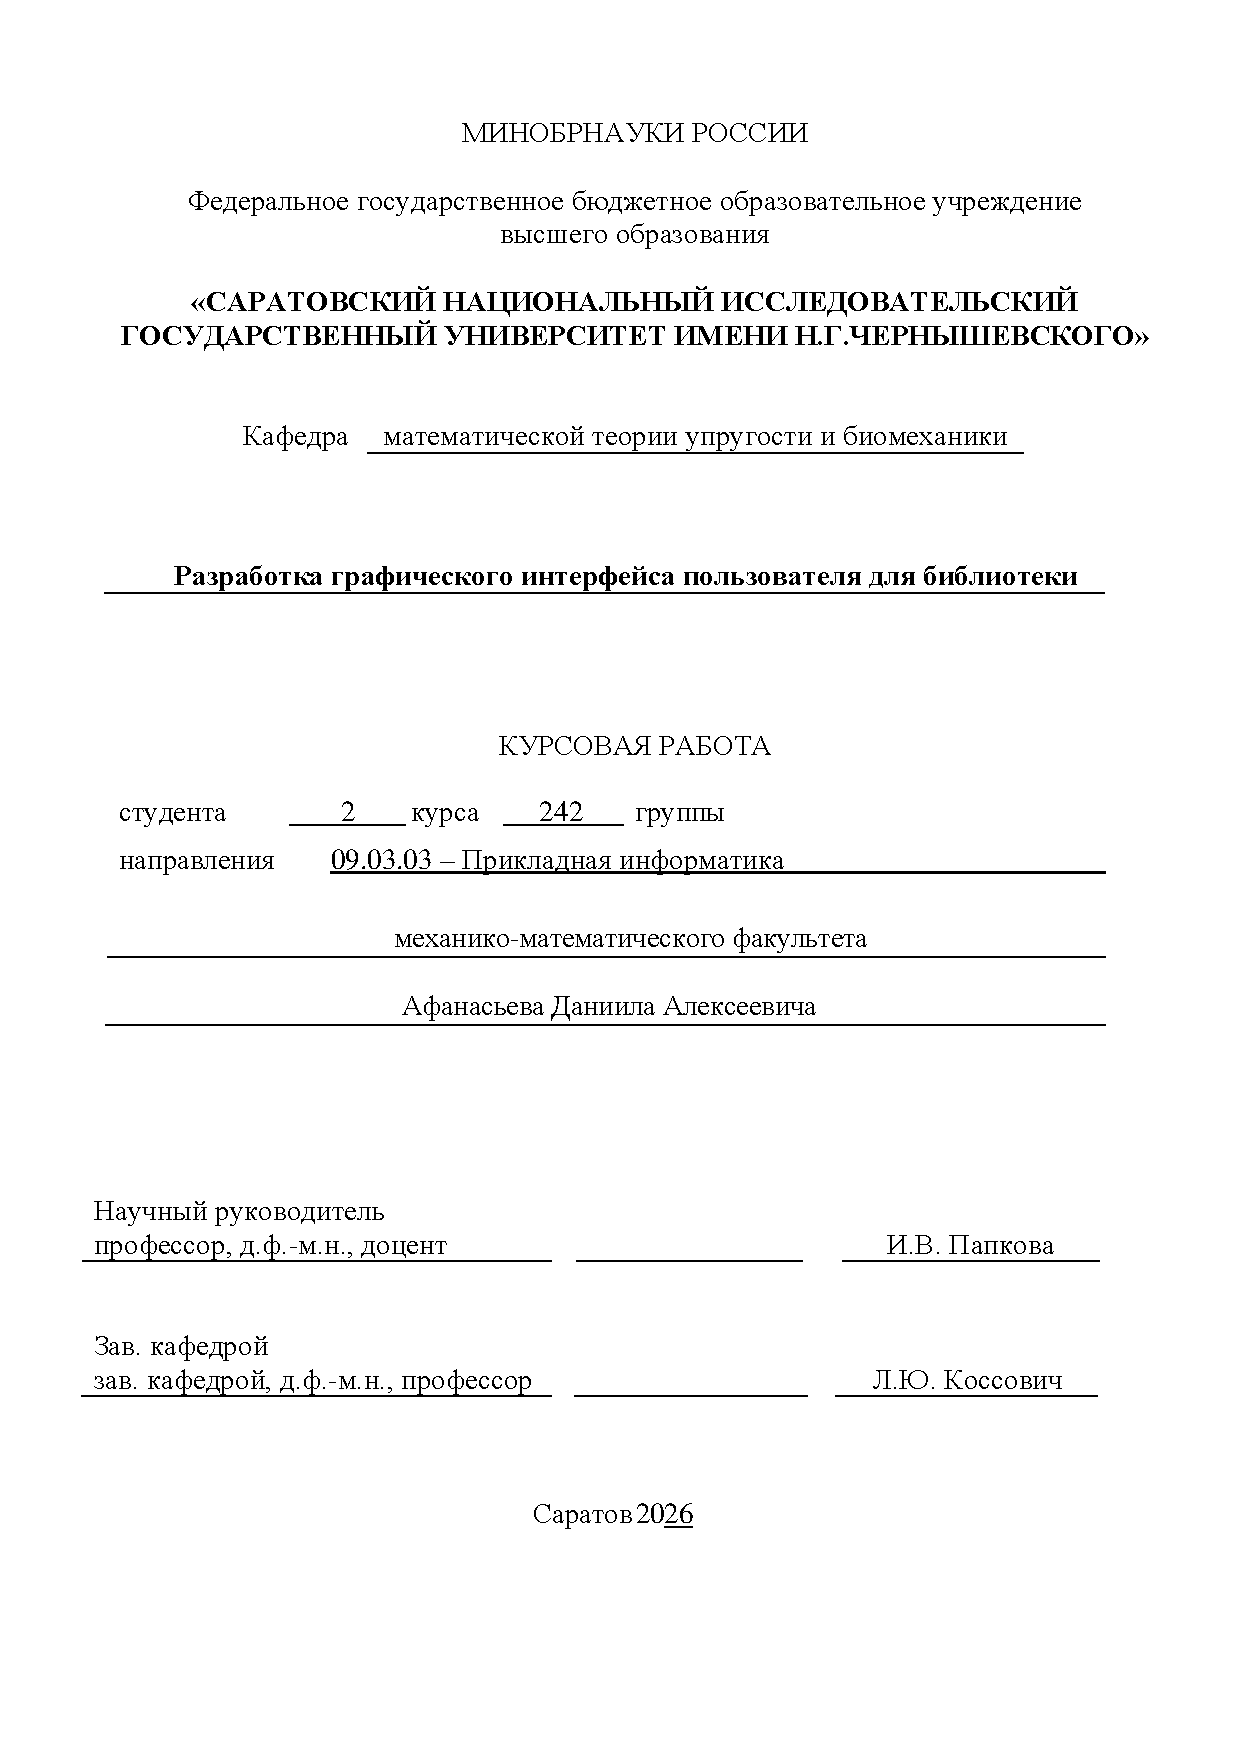
\includepdf[pages={1}]{Titulny_list_kursovoy_raboty.pdf}
	
	\tableofcontents
	
	\intro
	
	В современном мире автоматизация процессов управления становится неотъемлемой частью эффективной работы любой организации. Библиотеки, как учреждения, работающие с большим объёмом информации о книгах и читателях, особенно нуждаются в специализированных программных решениях. Применение информационных систем позволяет существенно сократить время на выполнение рутинных операций, снизить вероятность ошибок и обеспечить надёжное хранение данных.
	
	Актуальность данной работы обусловлена необходимостью автоматизации финансового учёта в библиотеке, предоставляющей книги напрокат. Ручное ведение записей о выданных книгах, залоговых суммах и платежах за прокат сопряжено с высоким риском ошибок и значительными временными затратами. Разработка графического интерфейса пользователя (GUI) на основе современных технологий позволяет решить эти проблемы~\cite{bib1}.
	
	Целью данной работы является разработка десктопного приложения с графическим интерфейсом для автоматизации учёта проката книг в библиотеке, включая управление фондом книг, картотекой читателей и финансовыми показателями.
	
	Для достижения цели решаются следующие задачи:
	\begin{itemize}
		\item анализ предметной области и проектирование структуры базы данных;
		\item разработка диаграмм UML и ER для формализации требований;
		\item реализация модуля работы с базой данных на языке Python;
		\item разработка графического интерфейса с использованием библиотеки PyQt5;
		\item тестирование функциональности приложения.
	\end{itemize}
	
	В разделе~1 описывается проектирование базы данных и приводится ER-диаграмма. В разделе~2 рассматриваются функциональные требования к системе с использованием UML-диаграммы вариантов использования. В разделе~3 описывается реализация приложения. В разделе~4 рассматривается структура интерфейса. Раздел~5 посвящён тестированию.
	
	
	\chapter{Проектирование базы данных}
	
	\section{Анализ предметной области}

	Система предназначена для библиотеки, осуществляющей прокат книг на коммерческой основе. Такая модель работы предполагает взимание платы за пользование книгами и внесение залоговой суммы, возвращаемой при возврате книги в сохранности.
	
	Предметная область включает следующие сущности и процессы:
	
	Книги --- единицы фонда, которые могут быть выданы напрокат. Каждая книга характеризуется названием, автором, жанром, залоговой стоимостью (которая взимается при выдаче и возвращается при возврате), стоимостью проката (плата за пользование книгой) и количеством экземпляров. Библиотека может иметь несколько экземпляров одной книги, что требует контроля их доступности. При проектировании системы важно обеспечить механизм отслеживания количества свободных экземпляров в реальном времени.
	
	Читатели --- зарегистрированные клиенты библиотеки с анкетными данными (фамилия, имя, отчество, адрес, телефон). Ведение картотеки читателей позволяет идентифицировать клиентов, отслеживать историю их взаимодействия с библиотекой, формировать статистику наиболее активных пользователей. Также наличие контактных данных обеспечивает возможность связи с читателем в случае просрочки возврата книги.
	
	Жанры --- классификатор литературных жанров, используемый для категоризации книг. Система жанров облегчает поиск и систематизацию фонда, позволяет формировать отчёты о популярности различных категорий литературы. Классификация может включать такие жанры, как художественная литература, научная литература, детективы, фантастика и другие.
	
	Выдачи --- факты выдачи книги читателю с указанием дат выдачи и ожидаемого возврата. Каждая выдача связывает конкретную книгу с конкретным читателем и фиксирует временные рамки проката. Система должна обеспечивать контроль за своевременностью возврата и уведомлять о просроченных выдачах.
	
	Возвраты --- факты возврата книги с фиксацией суммы оплаченного проката. При возврате система рассчитывает стоимость проката на основе установленной для книги цены, фиксирует дату возврата и формирует запись о финансовой транзакции. Эти данные используются для формирования финансовой отчётности и анализа доходности библиотечного фонда.
	
	Основные бизнес-процессы, реализуемые системой:
	
	
	\begin{enumerate}
		\item Регистрация читателя --- внесение в систему данных нового клиента библиотеки.
		\item Пополнение фонда --- добавление новых книг с указанием всех необходимых характеристик.
		\item Выдача книги --- оформление проката с проверкой доступности экземпляров.
		\item Возврат книги --- приём книги, расчёт и фиксация оплаты проката.
		\item Формирование отчётности --- генерация отчётов о текущих выдачах и финансовых показателях.
	\end{enumerate}
	
	При анализе предметной области были выявлены следующие ограничения и правила:
	
	\begin{itemize}
		\item Книгу можно выдать только при наличии свободных экземпляров.
		\item Один читатель может иметь несколько активных выдач одновременно.
		\item Возврат книги возможен только после её выдачи, повторный возврат блокируется системой.
		\item Стоимость проката фиксируется на момент выдачи книги и не изменяется при возврате.
	\end{itemize}

	На рисунке~\ref{fig:er} представлена ER-диаграмма, отображающая структуру базы данных с таблицами и связями между ними.
	
	\begin{figure}[H]
		\centering
		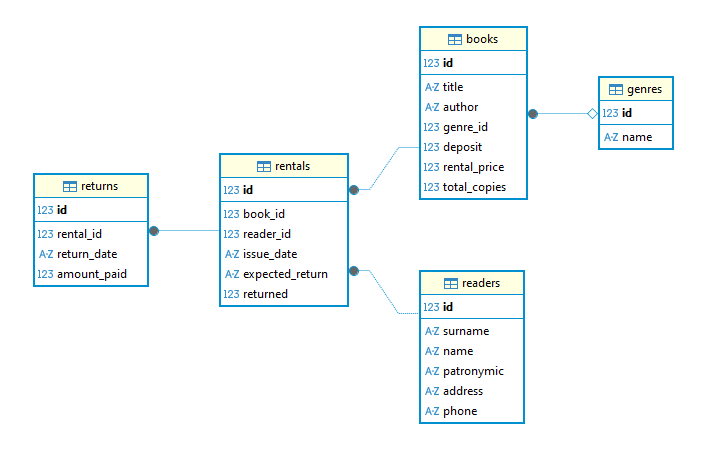
\includegraphics[width=0.85\textwidth]{images/er-diagrama.png}
		\caption{ER-диаграмма базы данных системы учёта проката книг}
		\label{fig:er}
	\end{figure}
	
	\section{Структура таблиц}
	
	База данных реализована в СУБД SQLite~\cite{bib2} и содержит пять таблиц.
	
	Таблица \texttt{genres} хранит жанры книг и содержит поля: \texttt{id} (первичный ключ, автоинкремент) и \texttt{name} (уникальное название жанра).
	
	Таблица \texttt{books} хранит сведения о книгах: \texttt{id}, \texttt{title} (название), \texttt{author} (автор), \texttt{genre\_id} (внешний ключ на таблицу жанров), \texttt{deposit} (залоговая стоимость), \texttt{rental\_price} (стоимость проката), \texttt{total\_copies} (общее количество экземпляров).
	
	Таблица \texttt{readers} содержит картотеку читателей: \texttt{id}, \texttt{surname}, \texttt{name}, \texttt{patronymic}, \texttt{address}, \texttt{phone}.
	
	Таблица \texttt{rentals} фиксирует факты выдачи книг: \texttt{id}, \texttt{book\_id} (внешний ключ), \texttt{reader\_id} (внешний ключ), \texttt{issue\_date} (дата выдачи), \texttt{expected\_return} (ожидаемая дата возврата), \texttt{returned} (флаг возврата).
	
	Таблица \texttt{returns} хранит финансовую историю возвратов: \texttt{id}, \texttt{rental\_id} (внешний ключ), \texttt{return\_date} (дата возврата), \texttt{amount\_paid} (сумма оплаты).
	
	В таблице~\ref{tab:relations} представлены связи между таблицами базы данных.
	
	\begin{table}[H]
		\caption{Связи между таблицами базы данных}
		\label{tab:relations}
		\begin{tabular}{|p{4cm}|p{4cm}|p{5cm}|}
			\hline
			\textbf{Таблица} & \textbf{Связанная \newline таблица} & \textbf{Тип связи} \\
			\hline
			genres & books & Один ко многим (один жанр --- много книг) \\
			\hline
			books & rentals & Один ко многим (одна книга --- много выдач) \\
			\hline
			readers & rentals & Один ко многим (один читатель --- много выдач) \\
			\hline
			rentals & returns & Один к одному (одна выдача --- один возврат) \\
			\hline
		\end{tabular}
	\end{table}
	
	Ссылочная целостность обеспечивается внешними ключами с политиками \texttt{ON UPDATE CASCADE} и \texttt{ON DELETE CASCADE} или \texttt{SET NULL}.
	
	
	\chapter{Моделирование функциональных требований}
	
	Основные варианты использования системы сгруппированы по функциональным областям.
	
	Управление жанрами: добавление нового жанра; редактирование названия жанра; удаление жанра; просмотр списка жанров.
	
	Управление книгами: добавление книги с указанием названия, автора, жанра, залоговой стоимости, стоимости проката и количества экземпляров; редактирование данных книги; удаление книги; просмотр каталога с информацией о доступных экземплярах.
	
	Управление читателями: регистрация нового читателя; редактирование анкетных данных; удаление читателя из картотеки; просмотр списка читателей.
	
	Учёт выдачи книг: оформление выдачи книги читателю с указанием дат; оформление возврата книги с автоматическим расчётом суммы оплаты; просмотр текущих и завершённых выдач.
	
	Финансовый учёт и отчётность: просмотр истории возвратов и оплат; отчёт по текущим выдачам (книги на руках); отчёт по выручке в разрезе книг.
	
	Для формализации функциональных требований была построена диаграмма вариантов использования (UML Use Case Diagram)~\cite{bib3}, представленная на рисунке~\ref{fig:usecase}. Диаграмма визуализирует основные функции системы и их взаимосвязь с актором.
	
В системе определён один актор --- сотрудник библиотеки, который взаимодействует со всеми функциями приложения. Потенциально систему можно расширить, введя роли (администратор, бухгалтер) с разными уровнями доступа, но в текущей реализации все функции доступны единственному пользователю.	

\begin{figure}[H]
		\centering
		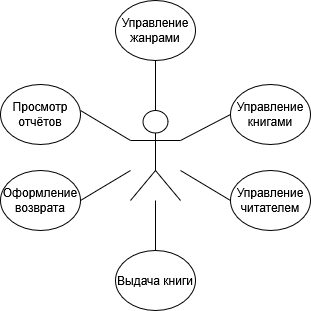
\includegraphics[width=0.85\textwidth]{images/uml.png}
		\caption{Диаграмма вариантов использования системы учёта проката книг}
		\label{fig:usecase}
	\end{figure}
	
	
	
	
	
	\section{Сценарии использования}
	
	Рассмотрим ключевые сценарии взаимодействия пользователя с системой.
	
	Сценарий 1: Выдача книги читателю.
	\begin{enumerate}
		\item Пользователь переходит на вкладку <<Выдачи>>.
		\item Нажимает кнопку <<Выдать книгу>>.
		\item В диалоговом окне выбирает книгу из списка доступных экземпляров.
		\item Выбирает читателя из картотеки.
		\item Указывает дату выдачи и ожидаемую дату возврата.
		\item Система сохраняет запись о выдаче в таблице \texttt{rentals}.
		\item Количество доступных экземпляров книги уменьшается на~1.
	\end{enumerate}
	
	Сценарий 2: Оформление возврата книги.
	\begin{enumerate}
		\item Пользователь выбирает активную запись о выдаче в таблице.
		\item Нажимает кнопку <<Оформить возврат>>.
		\item Система отображает информацию о книге, читателе и стоимости проката.
		\item После подтверждения фиксируется дата возврата, записывается сумма оплаты, статус выдачи обновляется на <<Возвращена>>.
		\item Таблица <<Возвраты>> обновляется автоматически.
	\end{enumerate}
	
	Сценарий 3: Просмотр финансового отчёта.
	\begin{enumerate}
		\item Пользователь переходит на вкладку <<Отчёты>>.
		\item Система отображает список книг, находящихся на руках у читателей.
		\item Система отображает сводную таблицу выручки по каждой книге.
		\item При необходимости пользователь нажимает <<Обновить отчёты>> для получения актуальных данных.
	\end{enumerate}
	
	
	\chapter{Реализация модуля базы данных}
	
	Приложение построено по принципу разделения ответственности~\cite{bib4} и состоит из двух основных модулей:
	\begin{itemize}
		\item \texttt{database.py} --- модуль для взаимодействия с базой данных SQLite; содержит класс \texttt{Database} с методами CRUD-операций для всех таблиц;
		\item \texttt{main\_qt.py} --- основной модуль приложения; содержит классы вкладок интерфейса и главного окна, реализованные средствами PyQt5.
	\end{itemize}
	
	Такая архитектура обеспечивает:
	\begin{itemize}
		\item Модульность: каждый компонент выполняет чётко определённую функцию.
		\item Тестируемость: слой данных можно тестировать независимо от интерфейса.
		\item Расширяемость: легко добавлять новые функции или изменять существующие без затрагивания других модулей.
		\item Повторное использование: класс Database можно использовать в других интерфейсах (например, веб-интерфейсе или консольном приложении).
	\end{itemize}

	Класс \texttt{Database} инкапсулирует все операции с базой данных~\cite{bib2}. При инициализации объекта вызывается метод \texttt{\_init\_db()}, который создаёт все таблицы при их отсутствии и наполняет базу тестовыми данными, если таблицы пусты.
	
	Метод \texttt{available\_copies(book\_id)} вычисляет количество доступных экземпляров книги путём вычитания числа невозвращённых выдач из общего количества экземпляров. Это позволяет предотвратить выдачу книги при отсутствии свободных экземпляров.
	
	Метод \texttt{process\_return(rental\_id, return\_date)} реализует бизнес-логику возврата: определяет стоимость проката конкретной книги, создаёт запись в таблице \texttt{returns} и обновляет флаг \texttt{returned} в таблице \texttt{rentals}. Метод возвращает сумму оплаты для отображения пользователю.
	
	Схема инициализации базы данных представлена ниже.
	
	\definecolor{bg}{rgb}{0.95,0.95,0.95}
	\begin{listing}[H]
		\begin{minted}[fontsize=\footnotesize,bgcolor=bg,baselinestretch=1.2,linenos,breaklines,frame=single]{sql}
			CREATE TABLE IF NOT EXISTS genres (
			id   INTEGER PRIMARY KEY AUTOINCREMENT,
			name TEXT NOT NULL UNIQUE
			);
			CREATE TABLE IF NOT EXISTS books (
			id           INTEGER PRIMARY KEY AUTOINCREMENT,
			title        TEXT NOT NULL,
			author       TEXT NOT NULL,
			genre_id     INTEGER REFERENCES genres(id) ON UPDATE CASCADE ON DELETE SET NULL,
			deposit      REAL NOT NULL DEFAULT 0,
			rental_price REAL NOT NULL DEFAULT 0,
			total_copies INTEGER NOT NULL DEFAULT 1
			);
			CREATE TABLE IF NOT EXISTS readers (
			id         INTEGER PRIMARY KEY AUTOINCREMENT,
			surname    TEXT NOT NULL,
			name       TEXT NOT NULL,
			patronymic TEXT NOT NULL DEFAULT '',
			address    TEXT NOT NULL DEFAULT '',
			phone      TEXT NOT NULL DEFAULT ''
			);
			CREATE TABLE IF NOT EXISTS rentals (
			id              INTEGER PRIMARY KEY AUTOINCREMENT,
			book_id         INTEGER NOT NULL REFERENCES books(id) ON DELETE CASCADE,
			reader_id       INTEGER NOT NULL REFERENCES readers(id) ON DELETE CASCADE,
			issue_date      TEXT NOT NULL,
			expected_return TEXT NOT NULL,
			returned        INTEGER NOT NULL DEFAULT 0
			);
			CREATE TABLE IF NOT EXISTS returns (
			id          INTEGER PRIMARY KEY AUTOINCREMENT,
			rental_id   INTEGER NOT NULL REFERENCES rentals(id) ON DELETE CASCADE,
			return_date TEXT NOT NULL,
			amount_paid REAL NOT NULL DEFAULT 0
			);
		\end{minted}
	\end{listing}
	
	Далее представлена реализация метода оформления возврата книги, который реализует ключевую финансовую логику приложения.
	
	\begin{listing}[H]
		\begin{minted}[fontsize=\footnotesize,bgcolor=bg,baselinestretch=1.2,linenos,breaklines,frame=single]{python}
			def process_return(self, rental_id: int, return_date: str) -> float:
			with self._connect() as conn:
			rental = conn.execute(
			"SELECT * FROM rentals WHERE id=?", (rental_id,)
			).fetchone()
			if not rental or rental['returned']:
			return 0.0
			book = conn.execute(
			"SELECT rental_price FROM books WHERE id=?",
			(rental['book_id'],)
			).fetchone()
			amount = book['rental_price'] if book else 0.0
			conn.execute(
			"INSERT INTO returns(rental_id, return_date, amount_paid)"
			" VALUES (?,?,?)",
			(rental_id, return_date, amount)
			)
			conn.execute(
			"UPDATE rentals SET returned=1 WHERE id=?", (rental_id,)
			)
			return amount
		\end{minted}
	\end{listing}
	
	
	\chapter{Реализация графического интерфейса}

	Графический интерфейс реализован с использованием библиотеки PyQt5~\cite{bib5}, которая предоставляет богатый набор виджетов и инструментов для создания кроссплатформенных приложений с нативным внешним видом. PyQt5 является набором привязок Python~\cite{bib6} к фреймворку Qt~\cite{bib7}. Данная библиотека обеспечивает полноценную интеграцию с операционными системами Windows, Linux и macOS, предоставляя единообразный программный интерфейс.
	
	Приложение содержит шесть вкладок:
	\begin{itemize}
		\item Жанры --- управление справочником литературных жанров. Данная вкладка позволяет добавлять новые категории книг, редактировать существующие названия и удалять неиспользуемые жанры.
		\item Книги --- управление каталогом книг с информацией о доступности. Здесь отображается полная информация о каждой книге: название, автор, жанр, залоговая стоимость, цена проката и общее количество экземпляров. Система автоматически вычисляет количество доступных для выдачи экземпляров.
		\item Читатели --- управление картотекой читателей. Вкладка содержит персональные данные всех зарегистрированных пользователей библиотеки, включая контактную информацию для связи.
		\item Выдачи --- учёт выдач книг и оформление возвратов. Это ключевая вкладка с точки зрения бизнес-процессов, здесь происходит основная работа с транзакциями проката.
		\item Возвраты --- история возвратов и финансовых операций. Вкладка предоставляет полную историю всех завершённых операций проката с указанием дат и сумм оплаты.
		\item Отчёты --- сводные отчёты по активным выдачам и выручке. Аналитический раздел, позволяющий контролировать финансовые показатели работы библиотеки.
	\end{itemize}
	
	Каждая вкладка использует вспомогательную функцию \texttt{make\_table()}, которая создаёт таблицу \texttt{QTableWidget}~\cite{bib5} с настроенными режимами отображения: запрет редактирования напрямую, выделение строк целиком, чередование цветов строк, автоматическое растяжение столбцов по ширине окна.
	
	Для добавления и редактирования записей используются модальные диалоговые окна (\texttt{QDialog}). В приложении реализованы следующие диалоги:
	\begin{itemize}
		\item GenreDialog --- ввод названия жанра;
		\item BookDialog --- ввод данных книги с выбором жанра из выпадающего списка;
		\item ReaderDialog --- ввод анкетных данных читателя;
		\item RentalDialog --- оформление выдачи с выбором книги и читателя, указанием дат.
	\end{itemize}
	
	На рисунке~\ref{fig:mainwindow} представлен внешний вид главного окна приложения.
	
	\begin{figure}[H]
		\centering
		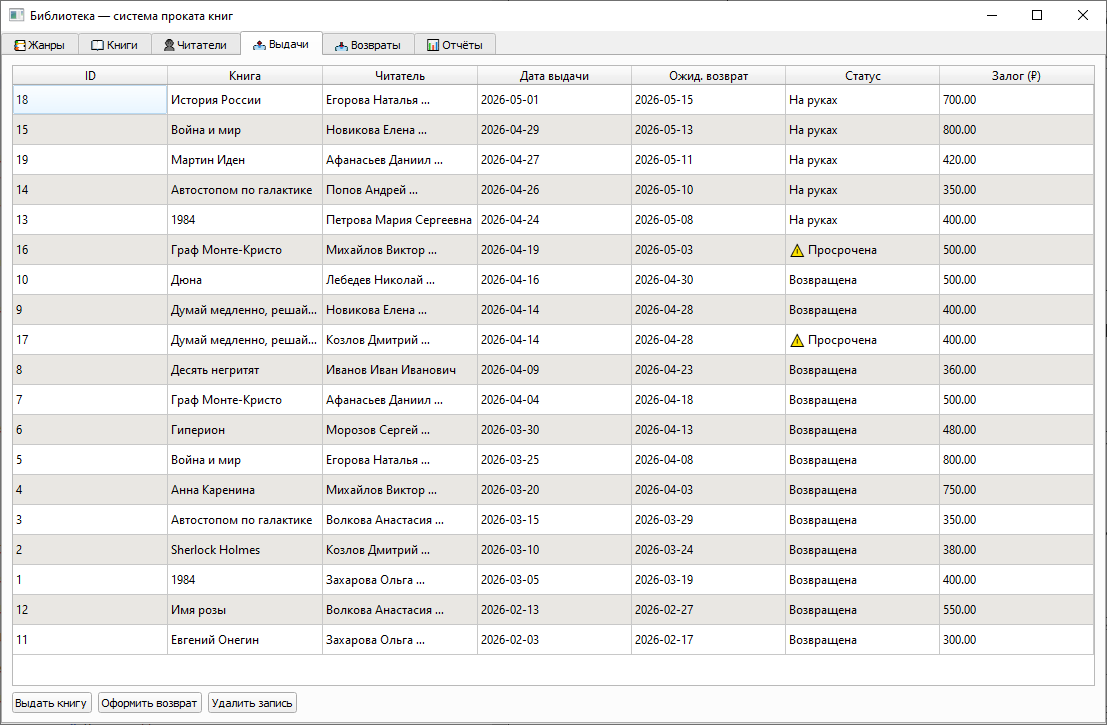
\includegraphics[width=0.85\textwidth]{images/Vidacha.png}
		\caption{Главное окно приложения, вкладка <<Выдачи>>}
		\label{fig:mainwindow}
	\end{figure}
	
	Вкладка <<Выдачи>> является ключевой с точки зрения бизнес-логики. В таблице отображаются все записи о выдачах с автоматическим расчётом статуса: <<Возвращена>>, <<На руках>> или <<Просрочена>> (если текущая дата превысила ожидаемую дату возврата).
	
	В диалоге выдачи книги в выпадающем списке отображаются только книги, у которых есть свободные экземпляры. При оформлении возврата производится запрос подтверждения с отображением суммы проката, после чего данные сохраняются в базе, а вкладка <<Возвраты>> обновляется автоматически.
	
	Вкладка <<Отчёты>> формирует два отчёта: текущие выдачи (книги на руках у читателей с указанием залогов) и сводную таблицу выручки в разрезе каждой книги по всем завершённым операциям проката.
	
	При переключении между вкладками данные автоматически обновляются благодаря подключению сигнала \texttt{currentChanged} вкладочного виджета к методу обновления активной вкладки.
	
	
	\chapter{Тестирование приложения}
	
	\section{Функциональное тестирование}
	
	В процессе разработки было проведено функциональное тестирование всех операций приложения. В таблице~\ref{tab:testing} приведены результаты тестирования ключевых функций.
	
	\begin{table}[H]
		\caption{Результаты функционального тестирования}
		\label{tab:testing}
		\begin{tabular}{|p{5.5cm}|p{5cm}|p{2.5cm}|}
			\hline
			\textbf{Тестируемая \newline функция} & \textbf{Ожидаемый \newline результат} & \textbf{Результат} \\
			\hline
			Добавление жанра & Запись сохраняется, список обновляется & Пройден \\
			\hline
			Добавление книги с жанром & Книга добавлена, связь с жанром установлена & Пройден \\
			\hline
			Регистрация читателя & Читатель добавлен в картотеку & Пройден \\
			\hline
			Выдача книги (есть экземпляр) & Запись создана, число доступных экз. уменьшилось & Пройден \\
			\hline
			Выдача (нет свободных экз.) & Книга не отображается в списке выдачи & Пройден \\
			\hline
			Оформление возврата & Запись создана, стоимость рассчитана верно & Пройден \\
			\hline
			Повторный возврат & Выдаётся предупреждение без изменения данных & Пройден \\
			\hline
			Отчёт по выручке & Отчёт содержит корректные суммы & Пройден \\
			\hline
			Просроченные выдачи & Статус <<Просрочена>> при нарушении срока & Пройден \\
			\hline
		\end{tabular}
	\end{table}
	
	\section{Тестирование защиты данных}
	
	Были проверены сценарии, связанные с обеспечением целостности данных. Попытка выдать книгу без свободных экземпляров блокируется на уровне интерфейса. Попытка повторно оформить возврат уже возвращённой книги вызывает информационное сообщение без изменения данных в базе. Ссылочная целостность таблиц поддерживается настройками внешних ключей SQLite с каскадным удалением зависимых записей.
	
	Все тесты успешно пройдены, приложение функционирует корректно и соответствует заявленным требованиям.
	
	\conclusions
	
	В ходе выполнения курсовой работы была разработана информационная система для автоматизации учёта проката книг в библиотеке. Достигнуты следующие результаты:
	
	\begin{enumerate}
		\item Проведён анализ предметной области, определены основные сущности: жанры, книги, читатели, выдачи и возвраты.
		\item Спроектирована реляционная база данных на основе СУБД SQLite~\cite{bib2,bib8}, состоящая из пяти взаимосвязанных таблиц с обеспечением ссылочной целостности посредством внешних ключей.
		\item Разработана ER-диаграмма базы данных~\cite{bib4} и диаграмма вариантов использования (UML Use Case)~\cite{bib3}, формализующая функциональные требования~\cite{bib9}.
		\item Реализован модуль \texttt{database.py}, инкапсулирующий все операции с базой данных, включая бизнес-логику расчёта стоимости проката при возврате.
		\item Разработан графический интерфейс пользователя на Python~\cite{bib6,bib10} с использованием библиотеки PyQt5~\cite{bib5}, организованный в виде шести тематических вкладок.
		\item Проведено функциональное тестирование, подтвердившее корректную работу всех реализованных функций.
	\end{enumerate}
	
	Созданное приложение позволяет автоматизировать учёт выдачи книг, отслеживать финансовые показатели проката (суммы залогов, стоимость проката, общую выручку) и контролировать своевременность возврата книг.
	
	Перспективы развития системы включают: добавление экспорта отчётов в форматы PDF и Excel; реализацию поиска и фильтрации; добавление функции уведомлений о просроченных выдачах; разработку веб-версии приложения.

	
	\begin{thebibliography}{10}
		
	\bibitem{bib1} Прохоренок, Н.~А. Python~3 и PyQt~5. Разработка приложений / Н.~А. Прохоренок. --- СПб. : БХВ-Петербург, 2016. --- 832~с.
	
	\bibitem{bib2} SQLite. SQLite Home Page [Электронный ресурс]. – URL:\url{https://www.sqlite.org/index.html} (дата обращения: 01.05.2026). - Загл. с экрана. - Яз. англ.
	
	\bibitem{bib3} Fowler, M. UML Distilled: A Brief Guide to the Standard Object Modeling Language / M.~Fowler. --- 3rd ed. --- Addison-Wesley Professional, 2004. --- 192~p. - Яз. англ.
	
	\bibitem{bib4} Коннолли, Т. Базы данных. Проектирование, реализация и сопровождение / Т.~Коннолли, К.~Бегг. --- 3-е изд. --- М. : Вильямс, 2003. --- 1440~с.
	
	\bibitem{bib5} Riverbank Computing Limited. PyQt5 Reference Guide [Электронный ресурс]. – URL:\url{https://www.riverbankcomputing.com/static/Docs/PyQt5/} (дата обращения: 01.05.2026). - Загл. с экрана. - Яз. англ.
	
	\bibitem{bib6} Python Software Foundation. Python~3 Documentation [Электронный ресурс]. – URL:\url{https://docs.python.org/3/} (дата обращения: 01.05.2026). - Загл. с экрана. - Яз. англ.
	
	\bibitem{bib7} Summerfield, M. Rapid GUI Programming with Python and Qt / M.~Summerfield. --- Addison-Wesley Professional, 2007. --- 648~p. - Яз. англ.
	
	\bibitem{bib8} Дейт, К.~Дж. Введение в системы баз данных / К.~Дж. Дейт. --- 8-е изд. --- М. : Вильямс, 2006. --- 1328~с.
	
	\bibitem{bib9} ГОСТ 34.602-89. Техническое задание на создание автоматизированной системы : Введ. 1990-01-01. --- М. : Издательство стандартов, 1989. --- 24~с.
	
	\bibitem{bib10} Культин, Н.~Б. Основы программирования в Python~3 / Н.~Б. Культин. --- СПб. : БХВ-Петербург, 2018. --- 288~с.
	
\end{thebibliography}

\end{document}